\chapter{Noticias relativas a: Malware en dispositivos móviles}

    % 1. Descripción y Título
    \section{Breve descripción de la amenaza: (más de 100 palabras)}
    La amenaza descrita se identifica como **SpyLoan**, 
    un tipo de malware financiero diseñado para 
    dispositivos móviles que opera bajo el esquema de 
    ``montadeudas''. Este software malicioso se disfraza 
    de aplicaciones legítimas de préstamos rápidos y 
    sin trámites burocráticos, dirigidas principalmente 
    a personas en situación de vulnerabilidad financiera. 
    Una vez instalada, la aplicación solicita permisos 
    excesivos y críticos, como acceso a la lista de 
    contactos, galería de fotos, ubicación GPS y 
    funciones de administración del sistema. 
    El objetivo es doble: por un lado, exfiltran 
    información personal sensible para realizar 
    extorsiones y acoso a los contactos del usuario; 
    por otro lado, el malware tiene la capacidad técnica 
    de bloquear remotamente el acceso al dispositivo 
    móvil del usuario si este no cumple con el pago de 
    intereses abusivos. Esta técnica de ``secuestro de 
    hardware'' convierte al teléfono inteligente en una 
    garantía forzosa, utilizando el control total sobre 
    el sistema operativo para coaccionar a la víctima, 
    lo que representa una evolución agresiva del 
    ransomware tradicional adaptado al ecosistema móvil.

    \section{Fecha de la noticia:}
    3 de diciembre de 2025
   
    \section{Título de la noticia:}
    \href{https://latam.kaspersky.com/about/press-releases/estafa-que-usa-celular-como-garantia-de-prestamo-se-expande-por-america-latina}{Estafa que usa celular como garantía de préstamo se expande por América Latina}

    % 2. Enlaces y Medio
    \section{Enlace a la noticia:}
    \href{https://latam.kaspersky.com/about/press-releases/estafa-que-usa-celular-como-garantia-de-prestamo-se-expande-por-america-latina}{https://latam.kaspersky.com/about/press-releases/estafa-que-usa-celular-como-garantia-de-prestamo-se-expande-por-america-latina}

    \section{Medio:}
    Kaspersky (Sala de Prensa Latam)
    
    \section{Enlace al medio:}
    \href{https://latam.kaspersky.com/}{https://latam.kaspersky.com/}

    \section{Nacionalidad del medio:}
    Internacional (Reporte específico para América Latina)
    
    \section{Idioma de la noticia:}
    Español
    
    \section{Pequeña imagen de la noticia:}
    \begin{center}
        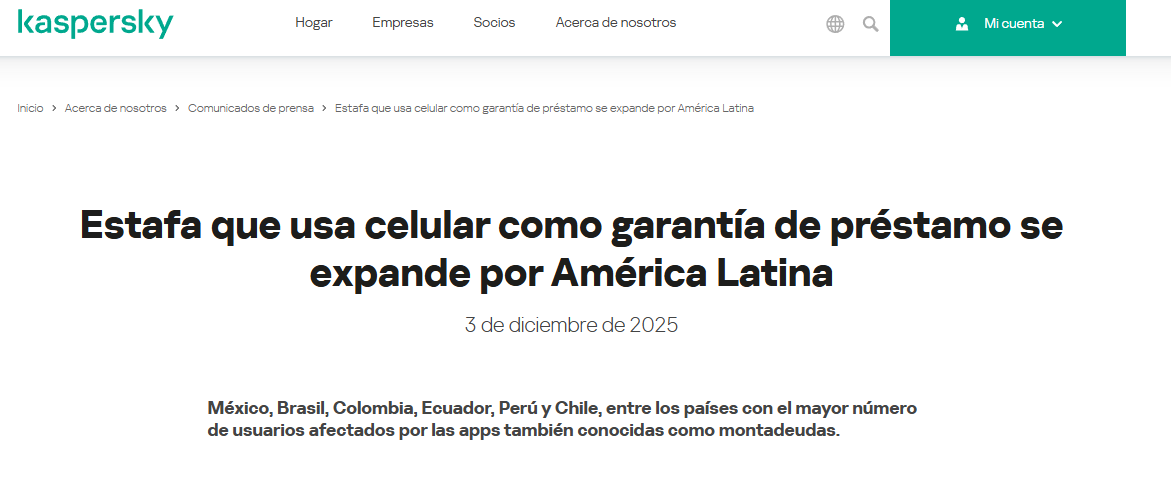
\includegraphics[width=0.8\textwidth]{Imagenes/06-malan.png} 
    \end{center} 

    % 4. Resumen y Análisis
    \section{Breve resumen de la noticia: (más de 100 palabras)}
    Un informe de Kaspersky revela una expansión masiva 
    de las aplicaciones maliciosas SpyLoan en América 
    Latina, registrando más de 521,000 bloqueos entre 
    agosto de 2024 y julio de 2025. México lidera el 
    ranking de afectados con 363,000 casos, seguido por 
    rasil y Colombia. Estas aplicaciones atraen a las 
    víctimas mediante anuncios en redes sociales 
    prometiendo crédito fácil. Una vez descargadas, 
    roban datos personales y bloquean los dispositivos 
    como método de extorsión ante el impago de deudas 
    con intereses usurarios. El reporte advierte además 
    sobre la aparición de un ``mercado paralelo'' 
    de supuestos hackers que ofrecen servicios para 
    desbloquear estos terminales, lo que supone un 
    riesgo adicional de infección por malware más 
    agresivo. Expertos de la firma de seguridad recalcan 
    que muchas de estas apps logran burlar los filtros 
    de las tiendas oficiales, por lo que recomiendan 
    limitar estrictamente los permisos de las aplicaciones, 
    mantener el sistema operativo actualizado y 
    desconfiar de ofertas financieras que no provengan 
    de instituciones legales reguladas.

    \section{Relación con la amenaza:}
    La noticia ilustra la convergencia entre el malware 
    móvil y la ingeniería social criminal. 
    SpyLoan utiliza funciones de administración 
    de dispositivos móviles (MDM) de forma maliciosa 
    para restringir el uso del dispositivo, convirtiéndolo 
    en un ``zombie'' bajo control del extorsionador.

    \section{\textquestiondown Existe CVE o CWE asociado a la noticia?}
    No se cita un CVE especifico.

    
    \section{Impacto ocasionado por la amenaza en esta noticia: (más de 100 palabras)}
    El impacto de SpyLoan es devastador tanto en el ámbito económico como en el personal. Financieramente, las víctimas se ven atrapadas en un ciclo de deuda impagable debido a intereses que superan la legalidad, sumado al costo de intentar recuperar el acceso a sus dispositivos. A nivel de privacidad, la filtración de listas de contactos permite a los criminales extender el acoso a familiares y amigos de la víctima, dañando su reputación y círculo social. El impacto técnico es crítico, ya que el bloqueo del dispositivo inutiliza una herramienta esencial para el trabajo y la comunicación. Además, el surgimiento de servicios fraudulentos de desbloqueo agrava la situación, pues los usuarios, en su desesperación, instalan más software malicioso que puede resultar en el robo total de cuentas bancarias y credenciales. Este fenómeno genera una desconfianza sistémica en las aplicaciones de tecnología financiera (Fintech) y resalta la vulnerabilidad de más de medio millón de usuarios en la región.